\documentclass[]{article}

\usepackage{listings}
\lstset{basicstyle=\ttfamily\footnotesize,breaklines=true}
\usepackage{graphicx}


% Title Page
\title{Uintah Portability Through Template Metaprogramming and Task Tagging}
\author{Brad Peterson}


\begin{document}
\maketitle
\section{Introduction}

Before Uintah's current template metaprogramming model, supporting CPUs and GPU tasks in the same build utilized an awkward mix of preprocessor ifdef statements, logical if statement branching, and special compile time options.  This process was not sustainable.  One attempted solution tried macros and automatic function call generation, but that again was becoming unwieldy and unsustainable.  A solution was found using template metaprogramming, and this document briefly describes its structure.

\section{Portability Needs}
\label{sec:portability_needs}
The list below summarizes desired needs from the perspective of both Uintah's runtime and application developers:

\begin{itemize}
\item Ease of use for application developers
\item Backwards compatibility with non-Kokkos tasks and loops
\item Multiple backend modes
\item Ease of adding additional future modes
\item Command line backend specific arguments (such as threads per loop)
\item Overriding these command line arguments within individual tasks
\item Multiple modes in the same compiled build
\begin{itemize}
\item Single build can run heterogeneous mixture of tasks: legacy, CPU only (e.g. solvers), GPU
\item Easier unit testing of modes (fewer builds needed)
\item Easier GPU debugging (Kokkos's nvcc\_wrapper terribly obfuscates source code.  So debug portable code for CPUs instead!)
\end{itemize}
\item Support task portability, not just loop portability
\begin{itemize}
\item Data warehouse retrieval should be portable
\item Need to write our own boundary conditions
\item Need our own portable variable initialization
\end{itemize}
\item Future possibility: Run tasks on both CPUs and GPUs simultaneously (most tasks are memory/latency bounded, could benefit from more buses)
\end{itemize}

\section{Core Pieces}

Template metaprogramming in Uintah did not come easy.  The significant challenge was that Uintah's runtime system which controlled task compilation was intertwined with C++ polymorphism.  Templates requires compile-time knowledge (i.e. early binding), and polymorphism requires runtime knowledge (i.e. late binding).  The cleanest solution was utilizing a parameter object to carry template parameters and template deduction.  This reduced the template metaprogramming to four core pieces, 1) task tagging, 2) a Uintah templated \emph{Execution Object}, 3) functors, and 4) task code.  These four are discussed in the following sections.

\subsection{Task Tagging}
\label{sec:task_tagging}
An application developer needs a mechanism to state which modes a task can support.  This process occurs at the point of code where the task is declared (in Uintah's case, that is in the task declaration code section which details the task requirements and its entry function).  

\begin{figure}[h]
	\centerline{
		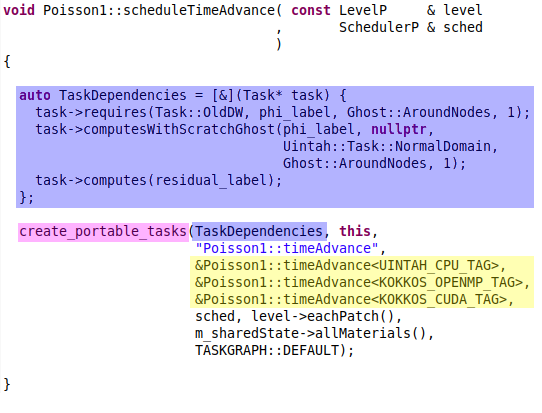
\includegraphics[width=0.8\textwidth,draft=false]{figures/poissonTaskAfter.png}
	}
	\caption{Task declaration with Uintah's new portable mechanisms.} 
	\label{fig:poisson_task_after}
\end{figure}

From the application developer's perspective, an example of task tagging is shown in Figure~\ref{fig:poisson_task_after}.  The yellow region in that figure is the key.  This mechanism marks the start of Uintah task template metaprogramming.   The tagged task template parameters propagate through several layers of Uintah, with propagation ending at the task code and task loops.  

The task tagging approach solves two core needs.  First, it allows the application developer to specify all possible modes the task supports.  Second, it helps ensure the compiler only compile the desired modes.  The key mechanism is the preprocessor defines for \texttt{UINTAH\_CPU\_TAG}, \texttt{KOKKOS\_OPENMP\_TAG}, and \texttt{KOKKOS\_CUDA\_TAG}. These three tags are defined in the Uintah runtime code as shown below:
\vspace{-0.05in}
\begin{lstlisting}
#define COMMA ,
#define UINTAH_CPU_TAG UintahSpaces::CPU COMMA UintahSpaces::HostSpace
#define KOKKOS_OPENMP_TAG Kokkos::OpenMP COMMA Kokkos::HostSpace
#define KOKKOS_CUDA_TAG Kokkos::Cuda COMMA Kokkos::CudaSpace
\end{lstlisting}

The C++ preprocessor expands the relevant portion of the Poisson code example into the following:
\vspace{-0.05in}
\begin{lstlisting}
create_portable_tasks( . . . , 
&Poisson1::timeAdvance<UintahSpaces::CPU, UintahSpaces::HostSpace>,
&Poisson1::timeAdvance<Kokkos::OpenMP, Kokkos::HostSpace>,
&Poisson1::timeAdvance<Kokkos::Cuda, Kokkos::CudaSpace>,
. . .)
\end{lstlisting}

That code would then attempt to compile three different flavors of the templated function \texttt{Poisson1::timeAdvance<>()}.   Note that the first template argument is the execution space, and the second template argument is the memory space.  


\subsubsection{Conditional Mode Compilation}

Suppose CUDA support was not desired.  Here, Uintah has a configure time define which demotes the CUDA tag into the following (note the third line changing to OpenMP):

\begin{lstlisting}
#define COMMA ,
#define UINTAH_CPU_TAG UintahSpaces::CPU COMMA UintahSpaces::HostSpace
#define KOKKOS_OPENMP_TAG Kokkos::OpenMP COMMA Kokkos::HostSpace
#define KOKKOS_CUDA_TAG Kokkos::OpenMP COMMA Kokkos::HostSpace
\end{lstlisting}

Now, the task declaration in Figure~\ref{fig:poisson_task_after} will be seen by the compiler as listing \texttt{\&Poisson1::timeAdvance<Kokkos::OpenMP, Kokkos::HostSpace>} twice, and so the compiler only compiles one of them.  Suppose Uintah is not configured with OpenMP or CUDA, then all three tags turn into \\ \texttt{\&Poisson1::timeAdvance<UintahSpaces::CPU, UintahSpaces::HostSpace>}, and so only 1 pthread mode is enabled.  Note that at the time of this writing, Uintah will only compile at most two of these in a single build, as OpenMP and pthreads do not mix well together.  


\subsection{Execution Object}

\begin{figure}[h]
	\centerline{
		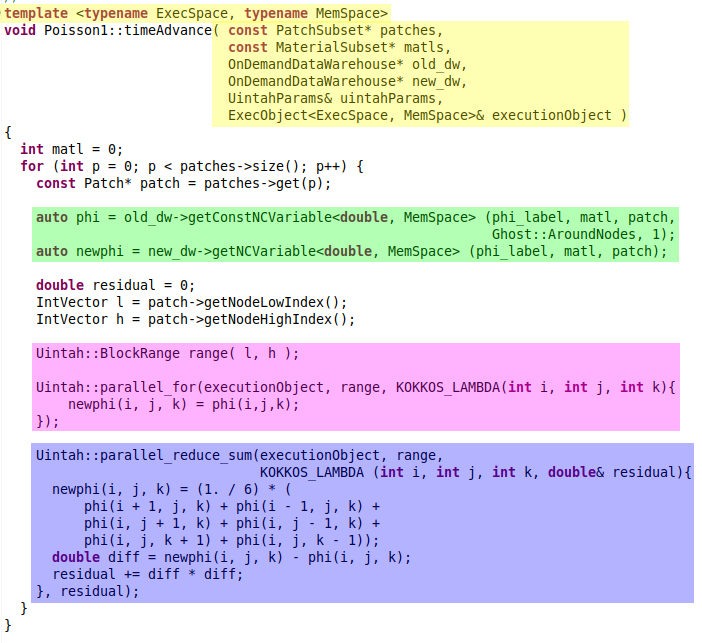
\includegraphics[width=1.0\textwidth,draft=false]{figures/poisson_task_code_after_colored.png}
	}
	\caption{ The portable Uintah Poisson task code capable of CPU and GPU compilation and execution.}
	\label{fig:poisson_task_code_after_colored}
\end{figure}

The \textbf{Execution Object} can be seen as the last argument of \texttt{timeAdvance} in Figure~\ref{fig:poisson_task_code_after_colored}.  This object carries with it the execution space and the memory space information, which were defined previously in Section~\ref{sec:task_tagging} in the task tagging phase.

A crucial piece is creating this Execution Object.  The process is best understood in the full flow, with the Execution object creation occurring in step 5c:

\begin{enumerate}
	\item{The \texttt{create\_portable\_tasks} is called (see Figure~\ref{fig:poisson_task_after}).   (Defined in \\ \texttt{Core/Parallel/TaskDeclaration.h}.)}  
	\item{The function creates a \texttt{Task} object for each execution space and memory space. (Defined in \texttt{Core/Grid/Task.h}.)}
	\begin{itemize}
		\item{The function also assigns a portable mode priority and launches the task in the appropriate backend}
		\item{The function also ensures that user placed tags (Section~\ref{sec:task_tagging}) does not require a specific order}
    \end{itemize}
    \item{The \texttt{Task} object carries template information and creates an \texttt{ActionPortable} object}
    \item{The \texttt{ActionPortable} stores the task function pointer address, preserving template parameters}
    \item{During execution:}
    \begin{enumerate} 
    	\item{A \texttt{DetailedTask} object is created, which inherits the \texttt{Task} class.}
    	\item{Uintah invokes a \texttt{DetailedTask} object's \texttt{do\_it()} method}
    	\item{The \texttt{do\_it()} method instantiates an \textbf{\texttt{ExecutionObject}}.  Template information is preserved as \texttt{do\_it()} is defined inside of \texttt{class ActionPortable}}
    	\item{The \texttt{ExecutionObject} is loaded with additional backend specific parameters}
    	\item{The \texttt{do\_it()} method calls \texttt{doit\_impl()}}
    	\item{The \texttt{doit\_impl()} method invokes the function pointer address}
    	\item{The application developer's task code executes with template information}
    \end{enumerate}
\end{enumerate}

For particular details, please refer to the specific code files themselves.  The prior list may seem too long at first glance, and the temptation is to find a way to shorten this list by reducing steps.  Unfortunately, the mixture of \texttt{DetailedTask}'s inheritance using late binding, with template metaprogramming's early binding, made the process difficult and necessitated each step.  Polymorphism can't carry template information.  Function pointers do not normally store template information either.  The key insight is to carry template information via a templated object in a function pointer.  


\subsection{Functors}

This section is somewhat obvious to experienced developers.  I mentioned it for two additional insights.  First, some forms of code portability are possible outside of functors, with OpenMP, OpenACC, OCCA, and Charm++ being prominent examples.  However, in my opinion, functors give Uintah the greatest overall cost vs. benefit net gain.  Second, functors allow Uintah to have portability outside of Kokkos, should such a need ever arise.  We do not need to lock ourselves into Kokkos's model.    

\subsection{Task Code}

The task code itself can now use the template parameters to aid in template metaprogramming.  Refer back to Figure~\ref{fig:poisson_task_code_after_colored}.  The data warehouse calls can be effectively overloaded to return a different type of object depending on the memory space templated argument used.  Note that the application developer uses the C++ \texttt{auto} keyword.  Normally, C++ does not allow overloading a function call by return type, but the concept works with template metaprogramming and \texttt{auto}.  

\begin{figure}[h]
	\centerline{
		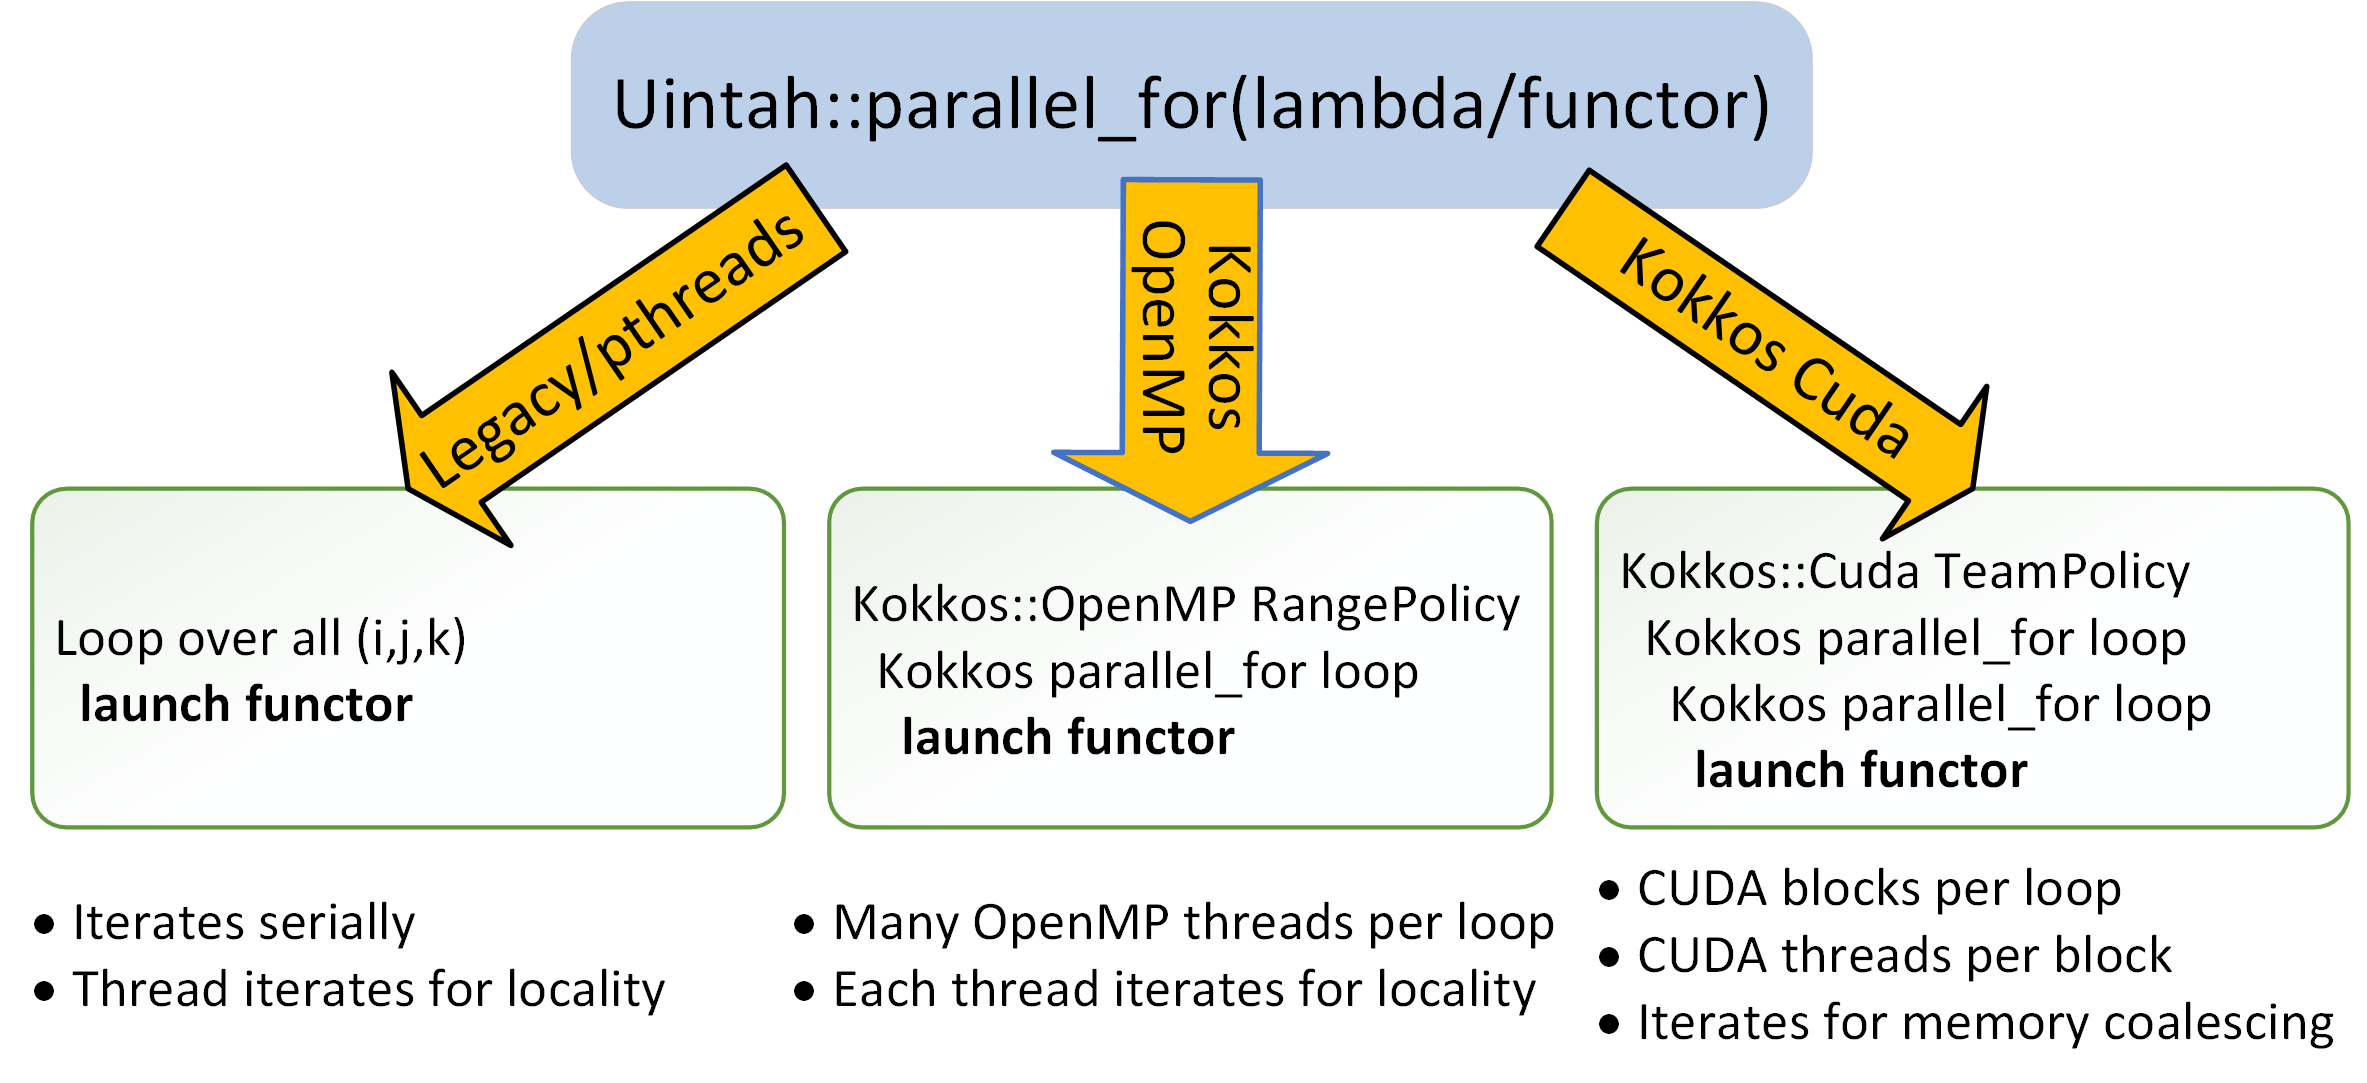
\includegraphics[width=1.0\textwidth,draft=false]{figures/uintah_parallel_for.png}
	}
	\caption{Uintah's \texttt{parallel\_for} supports three portable execution modes.} 
	\label{fig:uintah_parallel_for}
\end{figure}

Uintah's parallel loops avoid requiring template chevron syntax.  The Execution Object again carries the templated information.  Uintah relies on C++ template deduction to pass the template information.  Figure~\ref{fig:uintah_parallel_for} depicts how Uintah calls the correct parallel loop for the matching template execution space.  From here, Uintah is able to supply its own architecture specific backend loop options.  We found that Kokkos's portability options were insufficient for Uintah and we needed more control.  Further, we retain control to run our functors via pthreads in case Kokkos was not used at all.  

\subsection{Overview}

\begin{figure}[h]
	\centerline{
		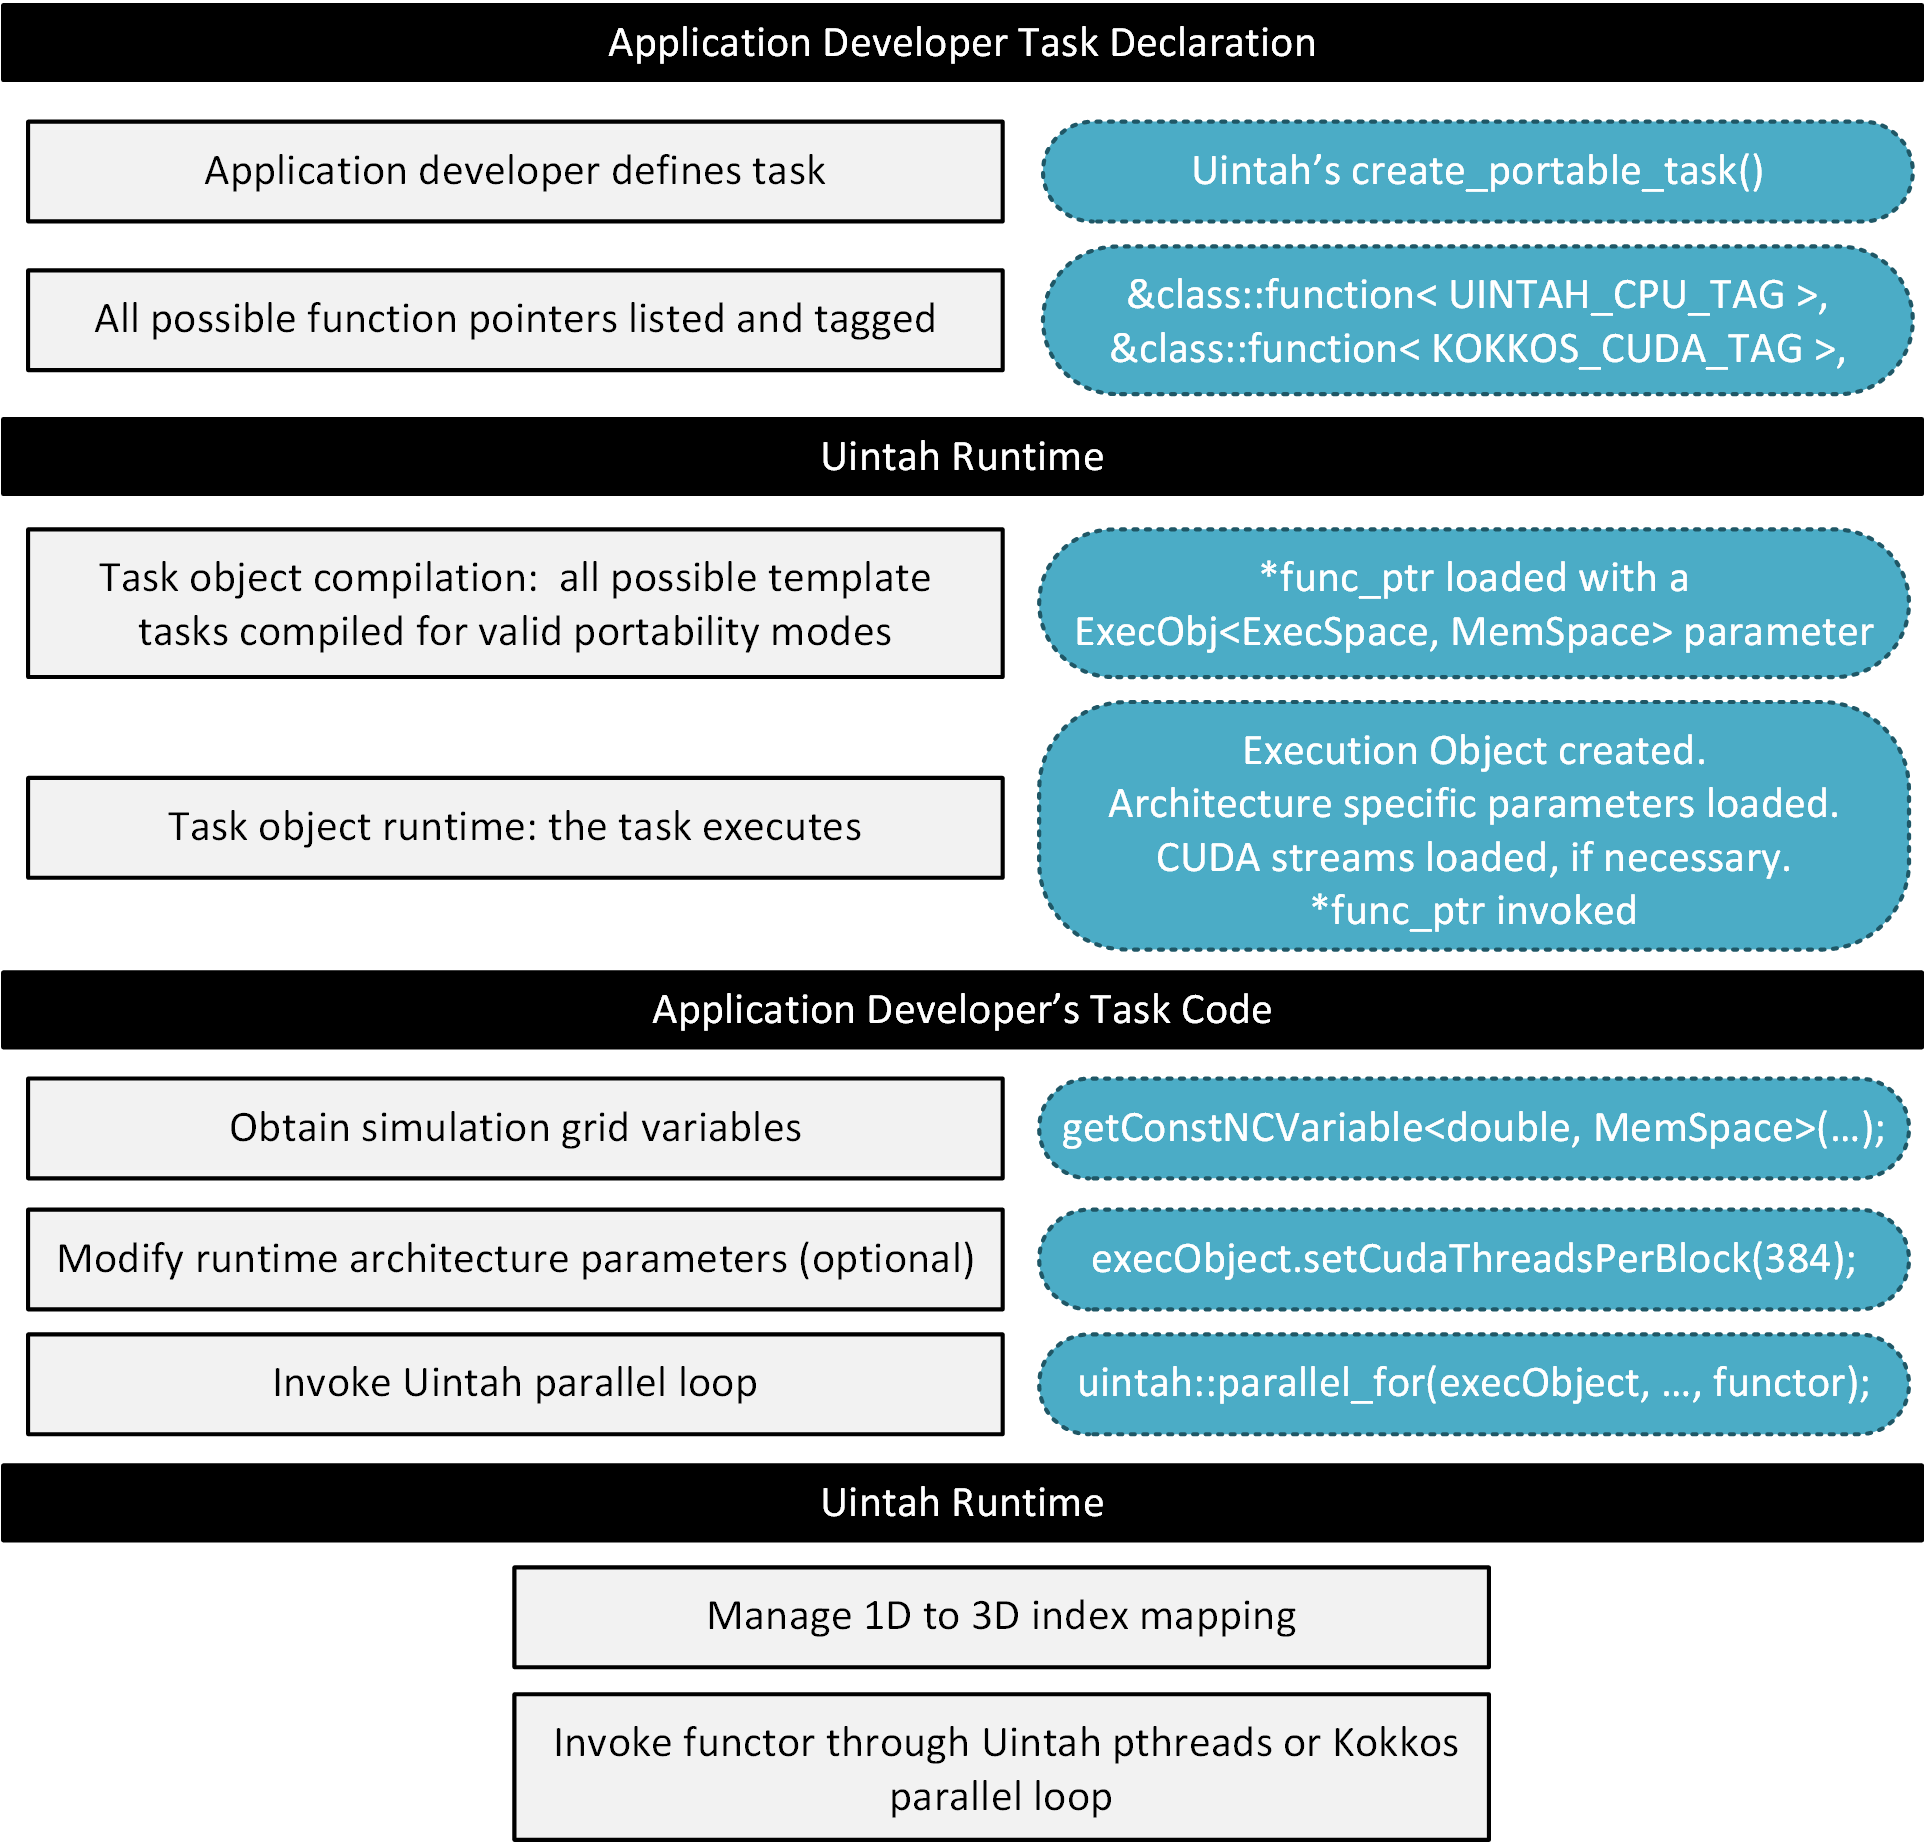
\includegraphics[width=1.0\textwidth,draft=false]{figures/template_metaprogramming.png}
	}
	\caption{Template metaprogramming of Uintah portable code starts at the task declaration phase, propagates into the runtime, then back into task code, then into Uintah's parallel API, then into Kokkos's parallel API.  The \emph{Execution Object} is a central piece of this template metaprogramming.} 
	\label{fig:template_metaprogramming}
\end{figure}

The process described thus far is also summarized in Figure~\ref{fig:template_metaprogramming}.

\section{Task Declaration, Configuration, Compilation, Runtime}

\begin{figure}[h]
	\centerline{
		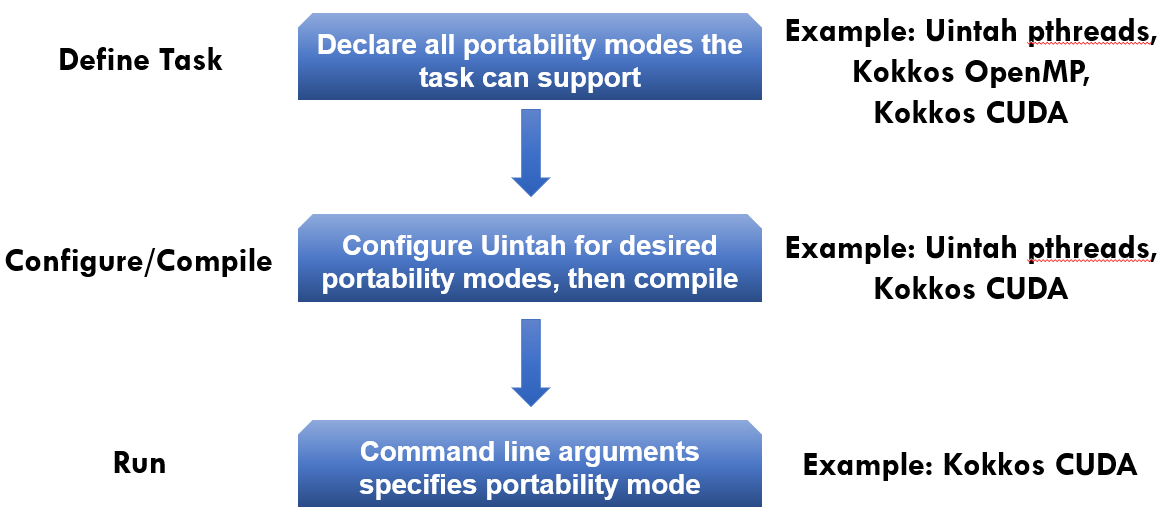
\includegraphics[width=1.0\textwidth,draft=false]{figures/portable_flow.png}
	}
	\caption{Tasks can be defined for many backends, compiled for a subset of these, and executed on only one of these.} 
	\label{fig:portable_flow}
\end{figure}

Another helpful way to understand Uintah's template metaprogramming  is to view the process in terms of building and using Uintah.  The task defines all possible modes that a particular task supports.  Uintah's configure script sets appropriate defines to tell all possible modes that should be supported at compilation, and likewise sets the defines that guard the appropriate tags (Section~\ref{sec:task_tagging}).  The compilation process then uses template parameters to ensure all desires modes are compiled, and thus tasks can be compiled for more than one backend.  The runtime process is controlled by Uintah command line arguments, and each task will only run on one backend.  A heterogeneous mix of tasks is easily supported, but an individual task itself cannot run on both CPUs and GPUs, for example.  The process described thus far is also summarized in Figure~\ref{fig:portable_flow}.

\section{Conclusion}

Uintah's template metaprogramming now supports the needs listed in Section~\ref{sec:portability_needs}.  Portability is easily managed by application developers by simply declaring modes a task can support.  Uintah supports heterogeneous tasks, and thus tasks can be tested and supported on new backends one-by-one.  Additionally, future portability modes are easily supported with just a few minor modifications, so that Uintah need not be locked into Kokkos, CUDA, OpenMP, or any other parallel programming model. 

\end{document}          
